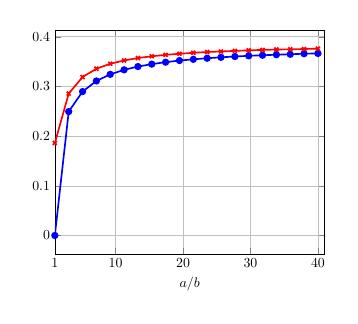
\begin{tikzpicture}[scale=0.5]
\begin{axis}[xlabel=$a/b$,ymajorgrids=true,xmajorgrids=true,xmin=1,xmax=41,xtick={1,10,20,30,40}]
%%%%%%%%%%% NATURAL CONFIGURATION
\addplot[Blue,mark=*,very thick] coordinates {(1.0,1.0000100001e-05) (3.05263157895,0.249310914162) (5.10526315789,0.28957342205) (7.15789473684,0.311013636452) (9.21052631579,0.324305874638) (11.2631578947,0.333392807612) (13.3157894737,0.339955504818) (15.3684210526,0.344870817129) (17.4210526316,0.348772961414) (19.4736842105,0.352087731404) (21.5263157895,0.354541966472) (23.5789473684,0.356753041215) (25.6315789474,0.358589375367) (27.6842105263,0.360175180699) (29.7368421053,0.361603616036) (31.7894736842,0.362721521952) (33.8421052632,0.363806269642) (35.8947368421,0.364694173258) (37.9473684211,0.365816289742) (40.0,0.366403664037) };
%%%%%%%%%%% MODIFIED CONFIGURATION
\addplot[Red,mark=x,very thick] coordinates {(1.0,0.186161861619) (3.05263157895,0.285515486734) (5.10526315789,0.318877925621) (7.15789473684,0.335565460918) (9.21052631579,0.345582403192) (11.2631578947,0.352315102098) (13.3157894737,0.357133045015) (15.3684210526,0.36070044911) (17.4210526316,0.363581004231) (19.4736842105,0.365719446668) (21.5263157895,0.367673150416) (23.5789473684,0.36925000829) (25.6315789474,0.37038001959) (27.6842105263,0.371525820521) (29.7368421053,0.372606357643) (31.7894736842,0.37353005109) (33.8421052632,0.374297427185) (35.8947368421,0.37474480008) (37.9473684211,0.375303226716) (40.0,0.376003760038) };
\end{axis}
\end{tikzpicture}
%%% Local Variables:
%%% mode: latex
%%% TeX-master: "../../mainManuscript"
%%% End:
